% Author: Izaak Neutelings (September 2018)
\documentclass[border=3pt,tikz]{standalone}
\usepackage{amsmath} % for \;
\usepackage{tikz}
\usepackage{xcolor}
\colorlet{myblue}{blue!70!black}
\colorlet{mylightblue}{blue!10}
\tikzset{>=latex} % for LaTeX arrow head
\usetikzlibrary{tikzmark} % for subnode

\begin{document}


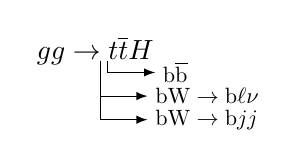
\begin{tikzpicture}[xscale=0.6,yscale=0.3,remember picture]
  \node (P) at (0,0) {$gg\to\subnode{t}{t}\overline{\subnode{tbar}{t}}\subnode{H}{H}$};
  \draw[->] (H.south)    |- +(1,-0.5) node[right,scale=0.8] {$\text{b}\overline{\text{b}}$};
  \draw[->] (tbar.south) |- +(1,-1.5) node[right,scale=0.8] {$\text{bW}\to\text{b}\ell\nu$};
  \draw[->] (t.south)    |- +(1,-2.5) node[right,scale=0.8] {$\text{bW}\to\text{b}jj$};
\end{tikzpicture}

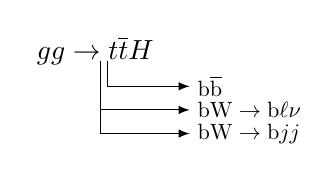
\begin{tikzpicture}[xscale=0.6,yscale=0.3,remember picture]
  \coordinate (t') at (2,-3.5);
  \coordinate (tbar') at (2,-2.5);
  \coordinate (H') at (2,-1.5);
  \node (P) at (0,0) {$gg\to\subnode{t1}{t}\overline{\subnode{tbar1}{t}}\subnode{H1}{H}$};
  \draw[->] (H1.south)    |- (H')    node[right,scale=0.8] {$\text{b}\overline{\text{b}}$};
  \draw[->] (tbar1.south) |- (tbar') node[right,scale=0.8] {$\text{bW}\to\text{b}\ell\nu$};
  \draw[->] (t1.south)    |- (t')    node[right,scale=0.8] {$\text{bW}\to\text{b}jj$};
\end{tikzpicture}

%\begin{tikzpicture}[yscale=0.8,anchor=west]
%  
%  % FIRST COLUMN
%  \node[anchor=west,draw=myblue,fill=mylightblue,thick,rounded corners=4,inner sep=1.5pt] (L) at (0,4) {\;\strut$qq\nu\nu$\;};  
%  \node (L1) at (0.5,3) {\strut$jj\nu\nu$};
%  \node (L2) at (0.5,2) {\strut bb$\nu\nu$};
%  \node (L3) at (0.5,1) {\strut tt$\nu\nu$};
%  \draw[->,myblue,thick] (L.south west)++(0.18,0) |- (L1.west);
%  \draw[->,myblue,thick] (L.south west)++(0.18,0) |- (L2.west);
%  \draw[->,myblue,thick] (L.south west)++(0.18,0) |- (L3.west);
%  
%  % SECOND COLUMN
%  \begin{scope}[shift={(2.5,0)}]
%    \node[draw=myblue,fill=mylightblue,thick,rounded corners=4,inner sep=1.5pt] (M) at (0,4) {\;\strut$qq\ell\ell$\;};
%    \node (M1) at (0.5,3) {\strut$jj\mu\mu$};
%    \node (M2) at (0.5,2) {\strut bb$\tau\tau$, b$\tau\tau$};
%    \node (M3) at (0.5,1) {\strut tt$\tau\tau$};
%    \draw[->,myblue,thick] (M.south west)++(0.18,0) |- (M1.west);
%    \draw[->,myblue,thick] (M.south west)++(0.18,0) |- (M2.west);
%    \draw[->,myblue,thick] (M.south west)++(0.18,0) |- (M3.west);
%  \end{scope}
%  
%  % THIRD COLUMN
%  \begin{scope}[shift={(5.0,0)}]
%    \node[draw=myblue,fill=mylightblue,thick,rounded corners=4,inner sep=1.5pt] (R) at (0,4) {\;\strut$qq\ell\nu$\;};
%    \node (R1) at (0.5,3) {\strut$jj\mu\nu$};
%    \draw[->,myblue,thick] (R.south west)++(0.18,0) |- (R1.west);
%  \end{scope}
%
%\end{tikzpicture}



\end{document}